\documentclass[aspectratio=169]{beamer}

% Language setup
\usepackage[magyar]{babel} % Babel for Hungarian
\usepackage[T1]{fontenc} % Output character encoding
\usepackage[utf8]{inputenc} % Input character encoding
\selectlanguage{magyar}

% Beamer styling setup
\usetheme{Boadilla}
\usecolortheme{default}
%\setbeamercolor{titlelike}{parent=structure,bg=gray!15}
\setbeamertemplate{navigation symbols}{}
\setbeamertemplate{caption}[numbered]
%

% Spacing setup
\setlength{\parindent}{0pt} % No paragraph indenting
\setlength{\parskip}{5pt} % Set spacing between paragraphs
\frenchspacing
\newcommand{\mkspace}{\vspace{19pt}}
\newcommand{\rmspace}{\vspace{-19pt}}
\newcommand{\emptyline}{\vspace{\baselineskip}}
%

% Dependency setup
\usepackage{tikz}
\usetikzlibrary{decorations.markings}
\usetikzlibrary{calc}
%

\usepackage{amsmath}


% Style setup
\usepackage{caption}
\usepackage{subcaption}
\captionsetup{format=plain, font=footnotesize, labelformat=empty}
\usepackage{colortbl}
%

% Notation setup
\usepackage{physics} % Braket notation

% Add qi.svg logo
\usepackage{svg}
\usepackage[absolute,overlay]{textpos}

% Newline in cell
\usepackage{makecell}

\author[Nemkin Viktória]{Nemkin Viktória}
\institute[]{
\begin{small}dr. Friedl Katalin\end{small}\\
\begin{footnotesize}Számítástudományi és Információelméleti Tanszék\end{footnotesize}
}
\title{Memóriafelhasználás optimalizálása}
\subtitle{kvantumalgoritmusok szimulációja során}
\date{}

\begin{document}

\begin{frame}
\titlepage

\begin{textblock*}{150pt}(280pt,200pt) % {block width} (coords)
\includesvg[inkscape=overwrite,width=150pt]{./figures/qi.svg}
\end{textblock*}
\end{frame}


\begin{frame}{Motiváció: "Protein folding" megoldása kvantumalgoritmussal}
\begin{columns}
\begin{column}{0.55\textwidth}
\begin{itemize}
    \item \textbf{Protein}:
    \begin{itemize}
        \item Aminosavakból alkotott lánc.
        \begin{itemize}
          \item \color{red} Piros = Hidrofób (''vízkerülő'').
          \item \color{blue} Kék = Poláris (''vízszerető'').
        \end{itemize}
        \item Hajtogatás: 3D kockarácson elhelyezés.
        \item Cél: Minimális energiájú elhelyezés megtalálása.
    \end{itemize}
    \item \textbf{Kódolás}:
    \begin{itemize}
        \item Origóból, lépésenként $6$ irány $=$ $6$ kvantumbit (qubit).
    \end{itemize}
    \item \textbf{Orákulum}: 
    \begin{itemize}
        \item Energiaviszonyok lepontozása.
    \end{itemize}
    \item \textbf{Grover keresés: $O(\sqrt{N})$}
    \begin{itemize}
        \item ''Kvantum párhuzamosság''-ot kihasználva.
        \item Energiaminimum megtalálása.
    \end{itemize}
\end{itemize}
\end{column}
\begin{column}{0.45\textwidth}
\begin{figure}[H]
\center
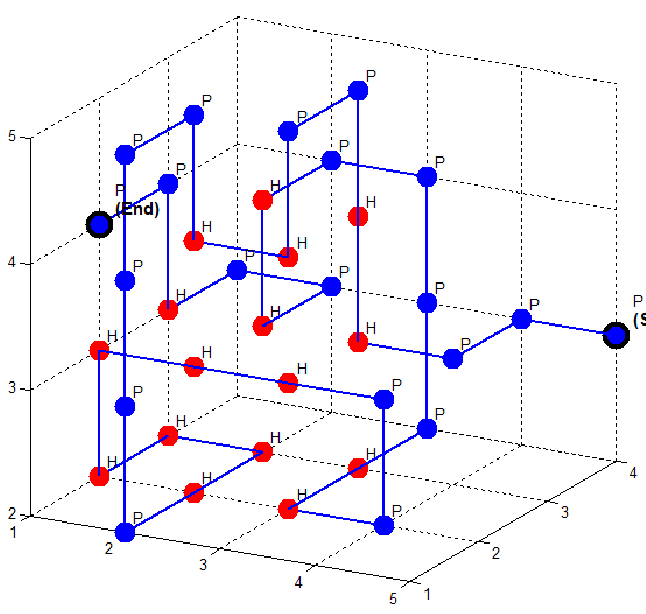
\includegraphics[width=\textwidth]{./figures/Protein-folds-with-length-36-amino-acids-18-contacts.png}
\caption{Egy összehajtogatott protein.}
\end{figure}
\end{column}
\end{columns}

\end{frame}

\begin{frame}[t]{Feladat}

\begin{itemize}
    \item \textbf{Cél}:
    \begin{itemize}
      \item Kvantumalgoritmusok kipróbálása és elemzése.
    \end{itemize}
    \item \textbf{Eszköztár}:
    \begin{itemize}
      \item Regiszterek.
      \item Operátorok: Hadamard, Grover, Sum, MC-NOT.
      \begin{itemize}
        \item ''Fekete doboz''-ként szimulálni.
      \end{itemize}
    \end{itemize}
    \item \textbf{Probléma}:
    \begin{itemize}
      \item Kvantumszámítógép: Publikusan nem elérhető (elég nagy).
      \item Klasszikus szimuláció: Túl sok memóriát fogyaszt.
    \end{itemize}
\end{itemize}
\end{frame}

\begin{frame}[t]{Probléma: Memóriahasználat}
\vspace{2mm}
\begin{tabular}{r|r|r|r}
Lánc & Qubitek & Regiszter & Operátor \\
\hline
\rule{0pt}{1.05\normalbaselineskip} $n$ & $6(n-1)$ & $2^{6(n-1)} \cdot{} 16 B$ & ${2^{12(n-1)}} \cdot{} 16 B$  \pause{} \\
\hline
2 & 6 &  1 KB &  64 KB \\
3 & 12 &  64 KB &  256 MB \\
4 & 18 &  4 MB & \color{red} \textbf{1 TB} \\
5 & 24 &  256 MB & \color{red} \textbf{4 PB} \\
6 & 30 &  16 GB & \color{red} \textbf{16384 PB} \\
7 & 36 & \color{red} \textbf{1 TB} & \color{red} \textbf{67108864 PB}
\end{tabular}
\pause
\vspace{2mm}
\begin{itemize}
    \item Optimalizációk (regiszer és operátor esetében is):
    \begin{itemize}
        \item Ritka mátrixos tárolás:
        \begin{itemize}
          \item IBM Qiskit, Google Cirq, stb.
          \item Nem mindig ritkák a mátrixok.
        \end{itemize}
        \item Döntési fa alapú adatszerkezet:
        \begin{itemize}
            \item Újabb kutatási irány.
            \item Nem mindig segít.
        \end{itemize}
    \end{itemize}
\end{itemize}

\end{frame}

\definecolor{applegreen}{rgb}{0.55, 0.71, 0.0}

\begin{frame}[t]{Megoldás: ''On-the-fly'' és ''Függvény-alapú'' operátorok}
\vspace{2mm}
\begin{tabular}{r|r|r|r|r|r}
Lánc & Qubitek & Regiszter & Operátor &  \cellcolor{applegreen!30} ''On-the-fly'' &  \cellcolor{applegreen!30} ''Függvény-alapú'' \\
\hline
\rule{0pt}{1.05\normalbaselineskip} $n$ & $6(n-1)$ & $2^{6(n-1)} \cdot{} 16 B$ & ${2^{12(n-1)}} \cdot{} 16 B$ &  = Regiszter. &   Nem kell tárolni. \\
\hline
2 & 6 &  1 KB &  64 KB &  1 KB & 0 B \\
3 & 12 &  64 KB &  256 MB &  64 KB & 0 B \\
4 & 18 &  4 MB & \color{red} \textbf{1 TB} &  4 MB & 0 B  \\
5 & 24 &  256 MB & \color{red} \textbf{4 PB} &  256 MB & 0 B \\
6 & 30 &  16 GB & \color{red} \textbf{16384 PB} &  16 GB & 0 B\\
7 & 36 & \color{red} \textbf{1 TB} & \color{red} \textbf{67108864 PB} & \color{red} \textbf{1 TB} & 0 B
\end{tabular}
\pause
\vspace{2mm}
\begin{itemize}
    \item Qiskit, stb. nyílt forráskódúak...
    \item ...de szerves része a kódnak az operátor tárolása
    \item $\rightarrow$ saját szimulátor implementáció.
\end{itemize}

\end{frame}


\begin{frame}{Regiszterek állapotának tárolása}

\begin{itemize}
    \item Minden bitsorozathoz egy komplex valószínűségi amplítúdó.
    \item Szuperpozíció és összefonódás $\rightarrow$ indexek Descartes-szorzata.
    \item Méretek: $2^{n_1}, \dots{}, 2^{n_s} \rightarrow \prod\limits_{i=1}^{s}2^{n_i}$.
\end{itemize}

\begin{columns}
\begin{column}{0.6\textwidth}
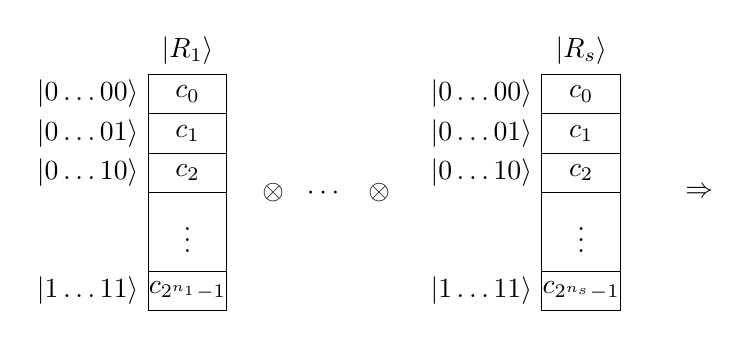
\begin{tikzpicture}

\def\start{0}
\def\w{1}
\def\h{0.5}

\node[anchor=south] at (\start+0.5*\w, \h) {$\ket{R_1}$};

\draw (\start,0) rectangle (\start+\w,\h);
\node[anchor=east] at (\start,0.5*\h) {$\ket{0\dots{}00}$};
\node[align=center] at (\start+0.5*\w,0.5*\h) {$c_0$};

\draw (\start,-1*\h) rectangle (\start+\w,0*\h);
\node[anchor=east] at (\start, -1*\h + 0.5*\h) {$\ket{0\dots{}01}$};
\node[align=center] at (\start + 0.5*\w, -1*\h + 0.5*\h) {$c_1$};

\draw (\start,-2*\h) rectangle (\start+\w,-1*\h);
\node[anchor=east] at (\start, -2*\h + 0.5*\h) {$\ket{0\dots{}10}$};
\node[align=center] at (\start + 0.5*\w, -2*\h + 0.5*\h) {$c_2$};

\draw (\start,-4*\h) rectangle (\start + \w,-2*\h);
\node[align=center] at (\start + 0.5*\w, -4*\h + \h) {$\vdots{}$};

\draw (\start,-5*\h) rectangle (\start + \w,-4*\h);
\node[anchor=east] at (\start, -5*\h + 0.5*\h) {$\ket{1\dots{}11}$};
\node[align=center] at (\start + 0.5*\w, -5*\h + 0.5*\h) {$c_{2^{n_1}-1}$};

% Dots


\node[align=center] at (2.3, -2*\h) {$\otimes{}~~\cdots{}~~\otimes{}$};

% Masodik

\def\start{5}

\node[anchor=south] at (\start+0.5*\w, \h) {$\ket{R_s}$};

\draw (\start,0) rectangle (\start+\w,\h);
\node[anchor=east] at (\start,0.5*\h) {$\ket{0\dots{}00}$};
\node[align=center] at (\start+0.5*\w,0.5*\h) {$c_0$};

\draw (\start,-1*\h) rectangle (\start+\w,0*\h);
\node[anchor=east] at (\start, -1*\h + 0.5*\h) {$\ket{0\dots{}01}$};
\node[align=center] at (\start + 0.5*\w, -1*\h + 0.5*\h) {$c_1$};

\draw (\start,-2*\h) rectangle (\start+\w,-1*\h);
\node[anchor=east] at (\start, -2*\h + 0.5*\h) {$\ket{0\dots{}10}$};
\node[align=center] at (\start + 0.5*\w, -2*\h + 0.5*\h) {$c_2$};

\draw (\start,-4*\h) rectangle (\start + \w,-2*\h);
\node[align=center] at (\start + 0.5*\w, -4*\h + \h) {$\vdots{}$};

\draw (\start,-5*\h) rectangle (\start + \w,-4*\h);
\node[anchor=east] at (\start, -5*\h + 0.5*\h) {$\ket{1\dots{}11}$};
\node[align=center] at (\start + 0.5*\w, -5*\h + 0.5*\h) {$c_{2^{n_s}-1}$};


% Rightarrow

\node[align=center] at (7, -2*\h) {$\Rightarrow$};

\end{tikzpicture}

\end{column}
\begin{column}{0.4\textwidth}

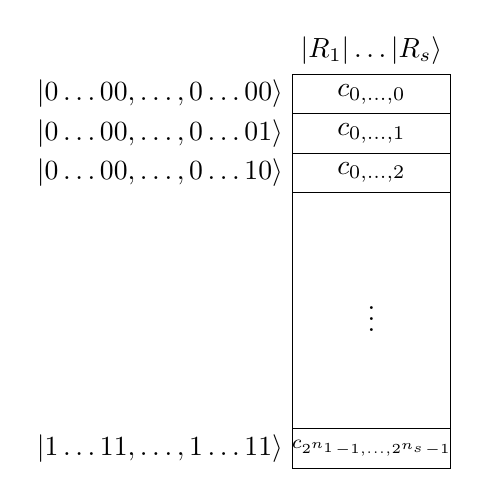
\begin{tikzpicture}
% Uccso osszes
\def\start{0}
\def\w{2}
\def\h{0.5}

\node[anchor=south] at (\start+0.5*\w, \h) {$\ket{R_1|\dots{}|R_s}$};

\draw (\start,0) rectangle (\start+\w,\h);
\node[anchor=east] at (\start,0.5*\h) {$\ket{0\dots{}00,\dots{},0\dots{}00}$};
\node[align=center] at (\start+0.5*\w,0.5*\h) {$c_{0,\dots{},0}$};

\draw (\start,-1*\h) rectangle (\start+\w,0*\h);
\node[anchor=east] at (\start, -1*\h + 0.5*\h) {$\ket{0\dots{}00,\dots{},0\dots{}01}$};
\node[align=center] at (\start + 0.5*\w, -1*\h + 0.5*\h) {$c_{0,\dots{},1}$};

\draw (\start,-2*\h) rectangle (\start+\w,-1*\h);
\node[anchor=east] at (\start, -2*\h + 0.5*\h) {$\ket{0\dots{}00,\dots{},0\dots{}10}$};
\node[align=center] at (\start + 0.5*\w, -2*\h + 0.5*\h) {$c_{0,\dots{},2}$};

\draw (\start,-8*\h) rectangle (\start + \w,-2*\h);
\node[align=center] at (\start + 0.5*\w, -6*\h + \h) {$\vdots{}$};

\draw (\start,-9*\h) rectangle (\start + \w,-8*\h);
\node[anchor=east] at (\start, -9*\h + 0.5*\h)  {$\ket{1\dots{}11,\dots{},1\dots{}11}$};
\node[align=center] at (\start + 0.5*\w, -9*\h + 0.5*\h) {\scriptsize$c_{2^{n_1}-1,\dots{}, 2^{n_s}-1}$};

\end{tikzpicture}
\end{column}
\end{columns}


\end{frame}

\begin{frame}{Regiszterkezelés nehézségei}

Példa: $A_{4\times{}4}$ ($2$ qubites) operátor.
\vspace{0.5cm}
\begin{columns}
  \begin{column}[t]{0.2\textwidth}
  \end{column}
  \begin{column}[t]{0.3\textwidth}
    \centering
    Utolsó 2 qubit-re:
    \begin{gather*}
      \ket{\square{}\dots{}\square{}\blacksquare{}\blacksquare{}} \\
      \Downarrow  \\
      \begin{pmatrix}
        A & 0  & \dots{} & 0 \\
       0 & A  & \dots{} & 0 \\ 
       \vdots{} & \vdots{}  & \ddots{} & \vdots{} \\
       0 & 0  & \dots{} & A \\
     \end{pmatrix} \\
     \searrow
    \end{gather*}
  \end{column}
  \begin{column}[t]{0.3\textwidth}
    \centering
    Első 2 qubit-re:
    \begin{gather*}
      \ket{\blacksquare{}\blacksquare{}\square{}\dots{}\square{}} \\
      \Downarrow \\
      \begin{pmatrix}
        A_{0,0} I & A_{0,1} I & A_{0,2} I & A_{0,3} I  \\
        A_{1,0} I & A_{1,1} I & A_{1,2} I & A_{1,3} I \\
        A_{2,0} I & A_{2,1} I & A_{2,2} I & A_{2,3} I \\
        A_{3,0} I & A_{3,1} I & A_{3,2} I & A_{3,3} I \\
      \end{pmatrix}\\[3pt]
     \swarrow
    \end{gather*}
  \end{column}
  \begin{column}[t]{0.2\textwidth}
  \end{column}
  \end{columns}

\begin{center}
  Köztes esetek?\\
  $\ket{\square{}\dots{}\square{}\blacksquare{}\square{}\dots{}\square{}\blacksquare{}\square{}\dots{}\square{}} $
\end{center}

\end{frame}

\begin{frame}{Qubit és index leképezés}

\vspace{0.25cm}
\textbf{Qubit map}
\vspace{-0.4cm}
\begin{figure}[H]
    \centering
    
\includegraphics[width=0.7\textwidth]{figures/qubit_mapping.png}
\end{figure}
\vspace{-0.4cm}
\textbf{Index map}
\vspace{-0.4cm}
\begin{figure}[H]
  \centering
  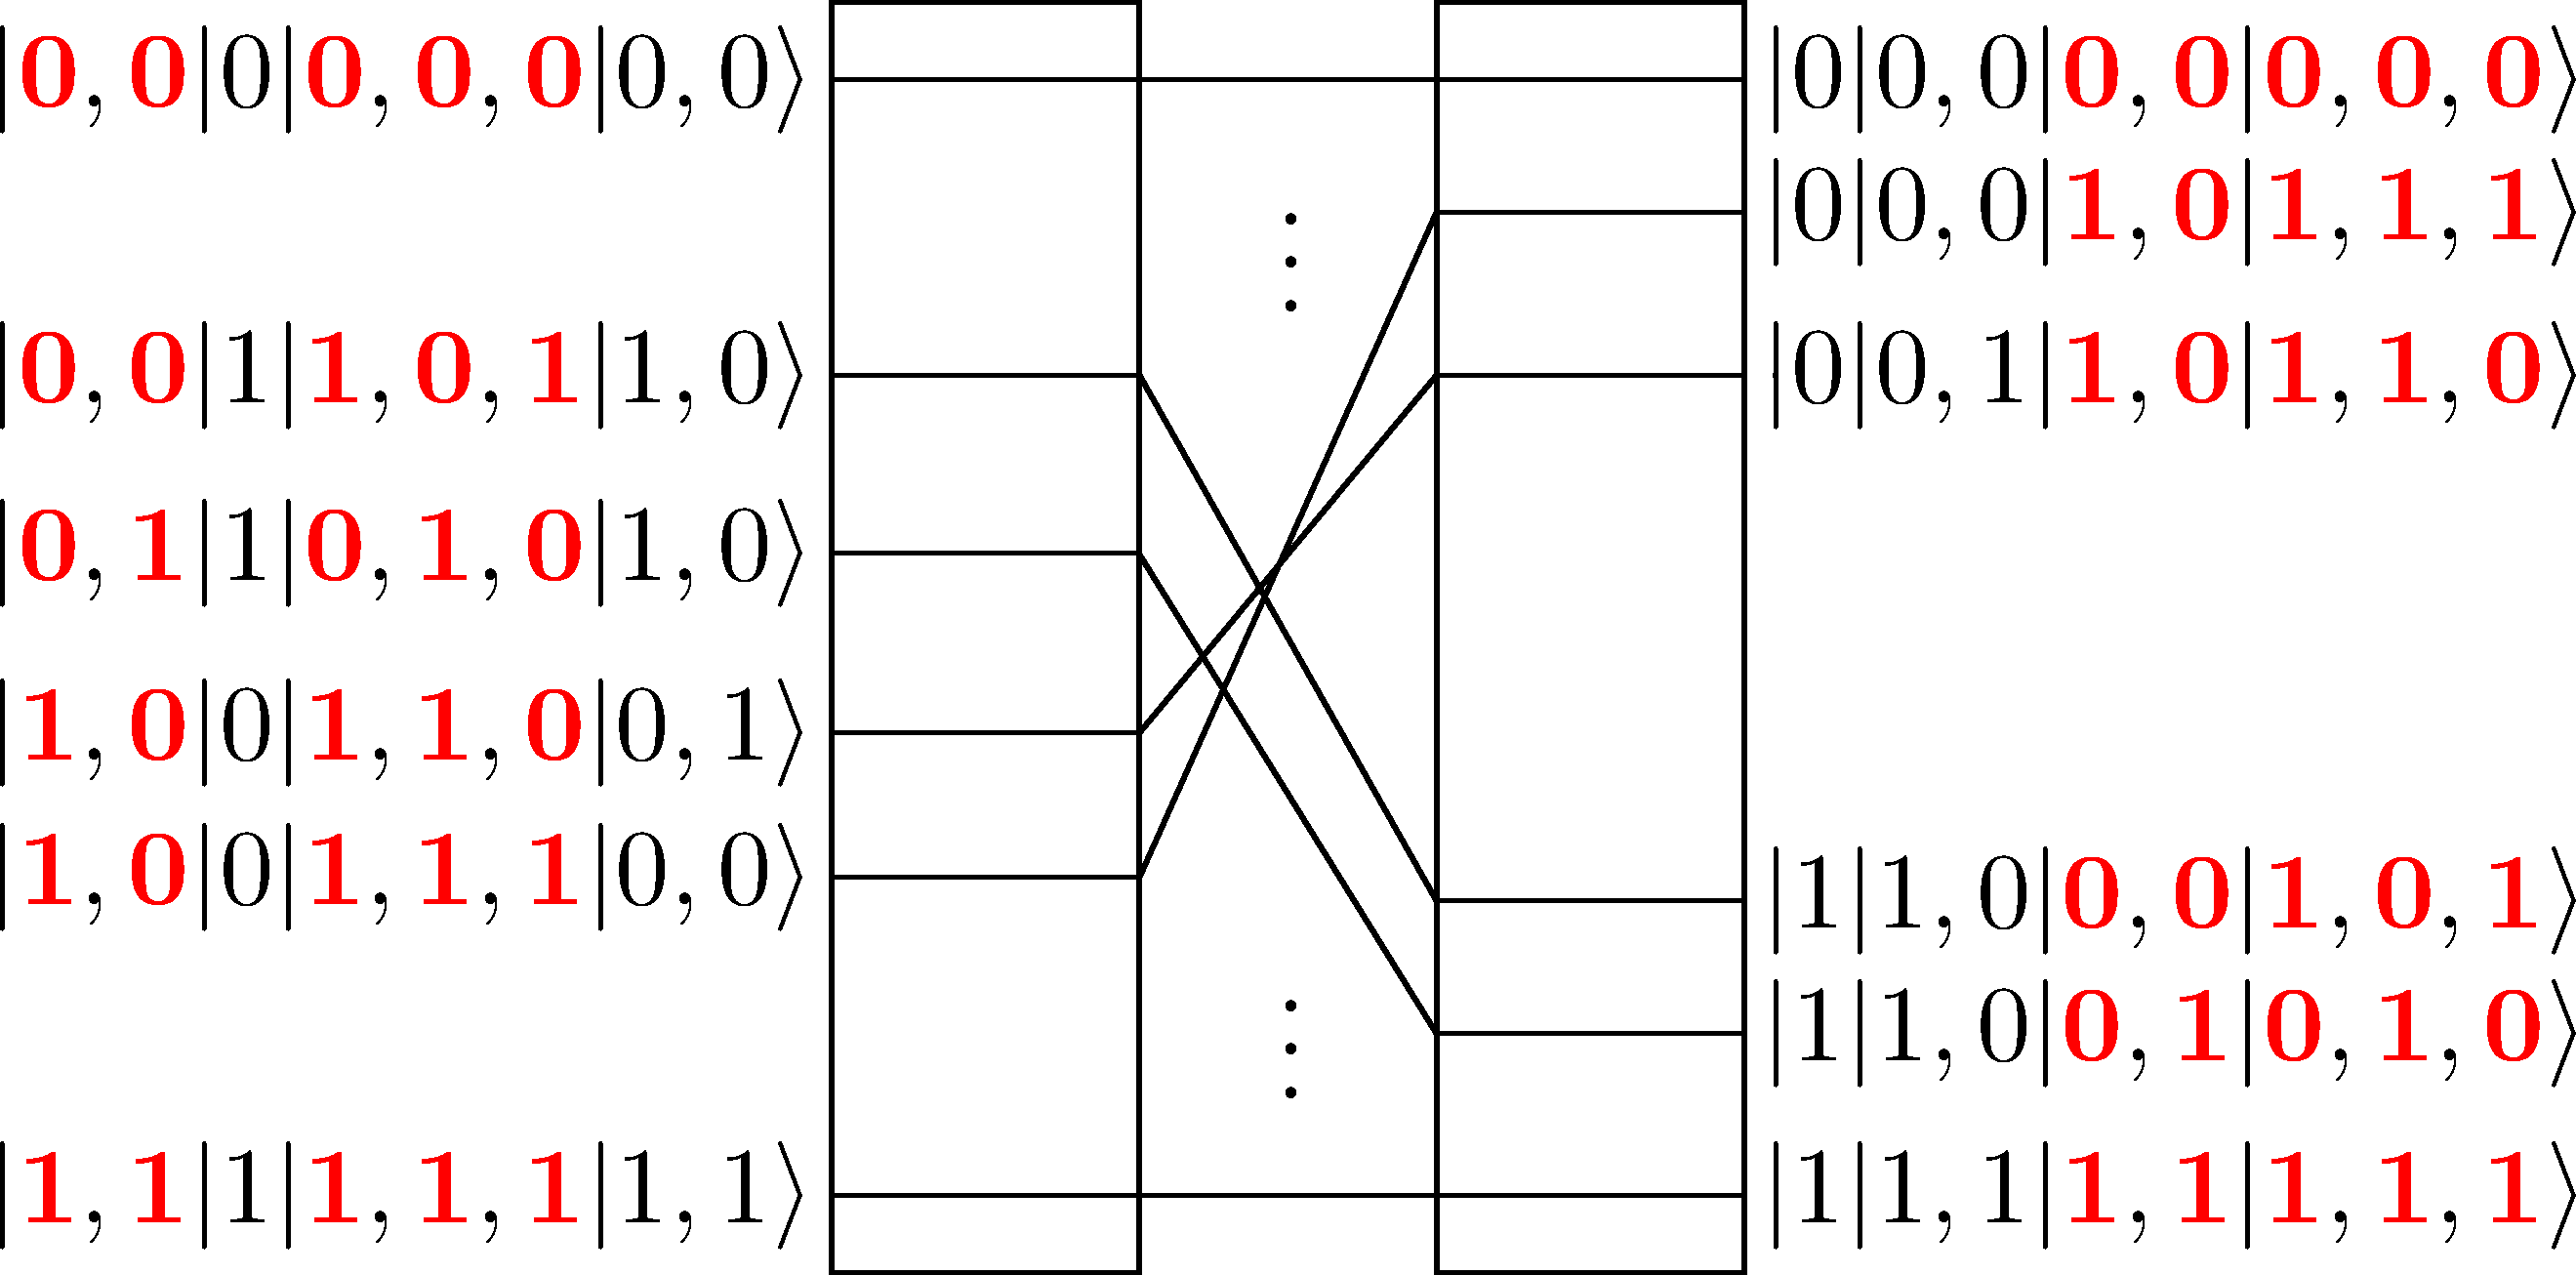
\includegraphics[width=0.7\textwidth]{figures/index_mapping.png}
\end{figure}

\end{frame}


\begin{frame}{Operátor végrehajtás}

\begin{figure}[H]
    \centering
    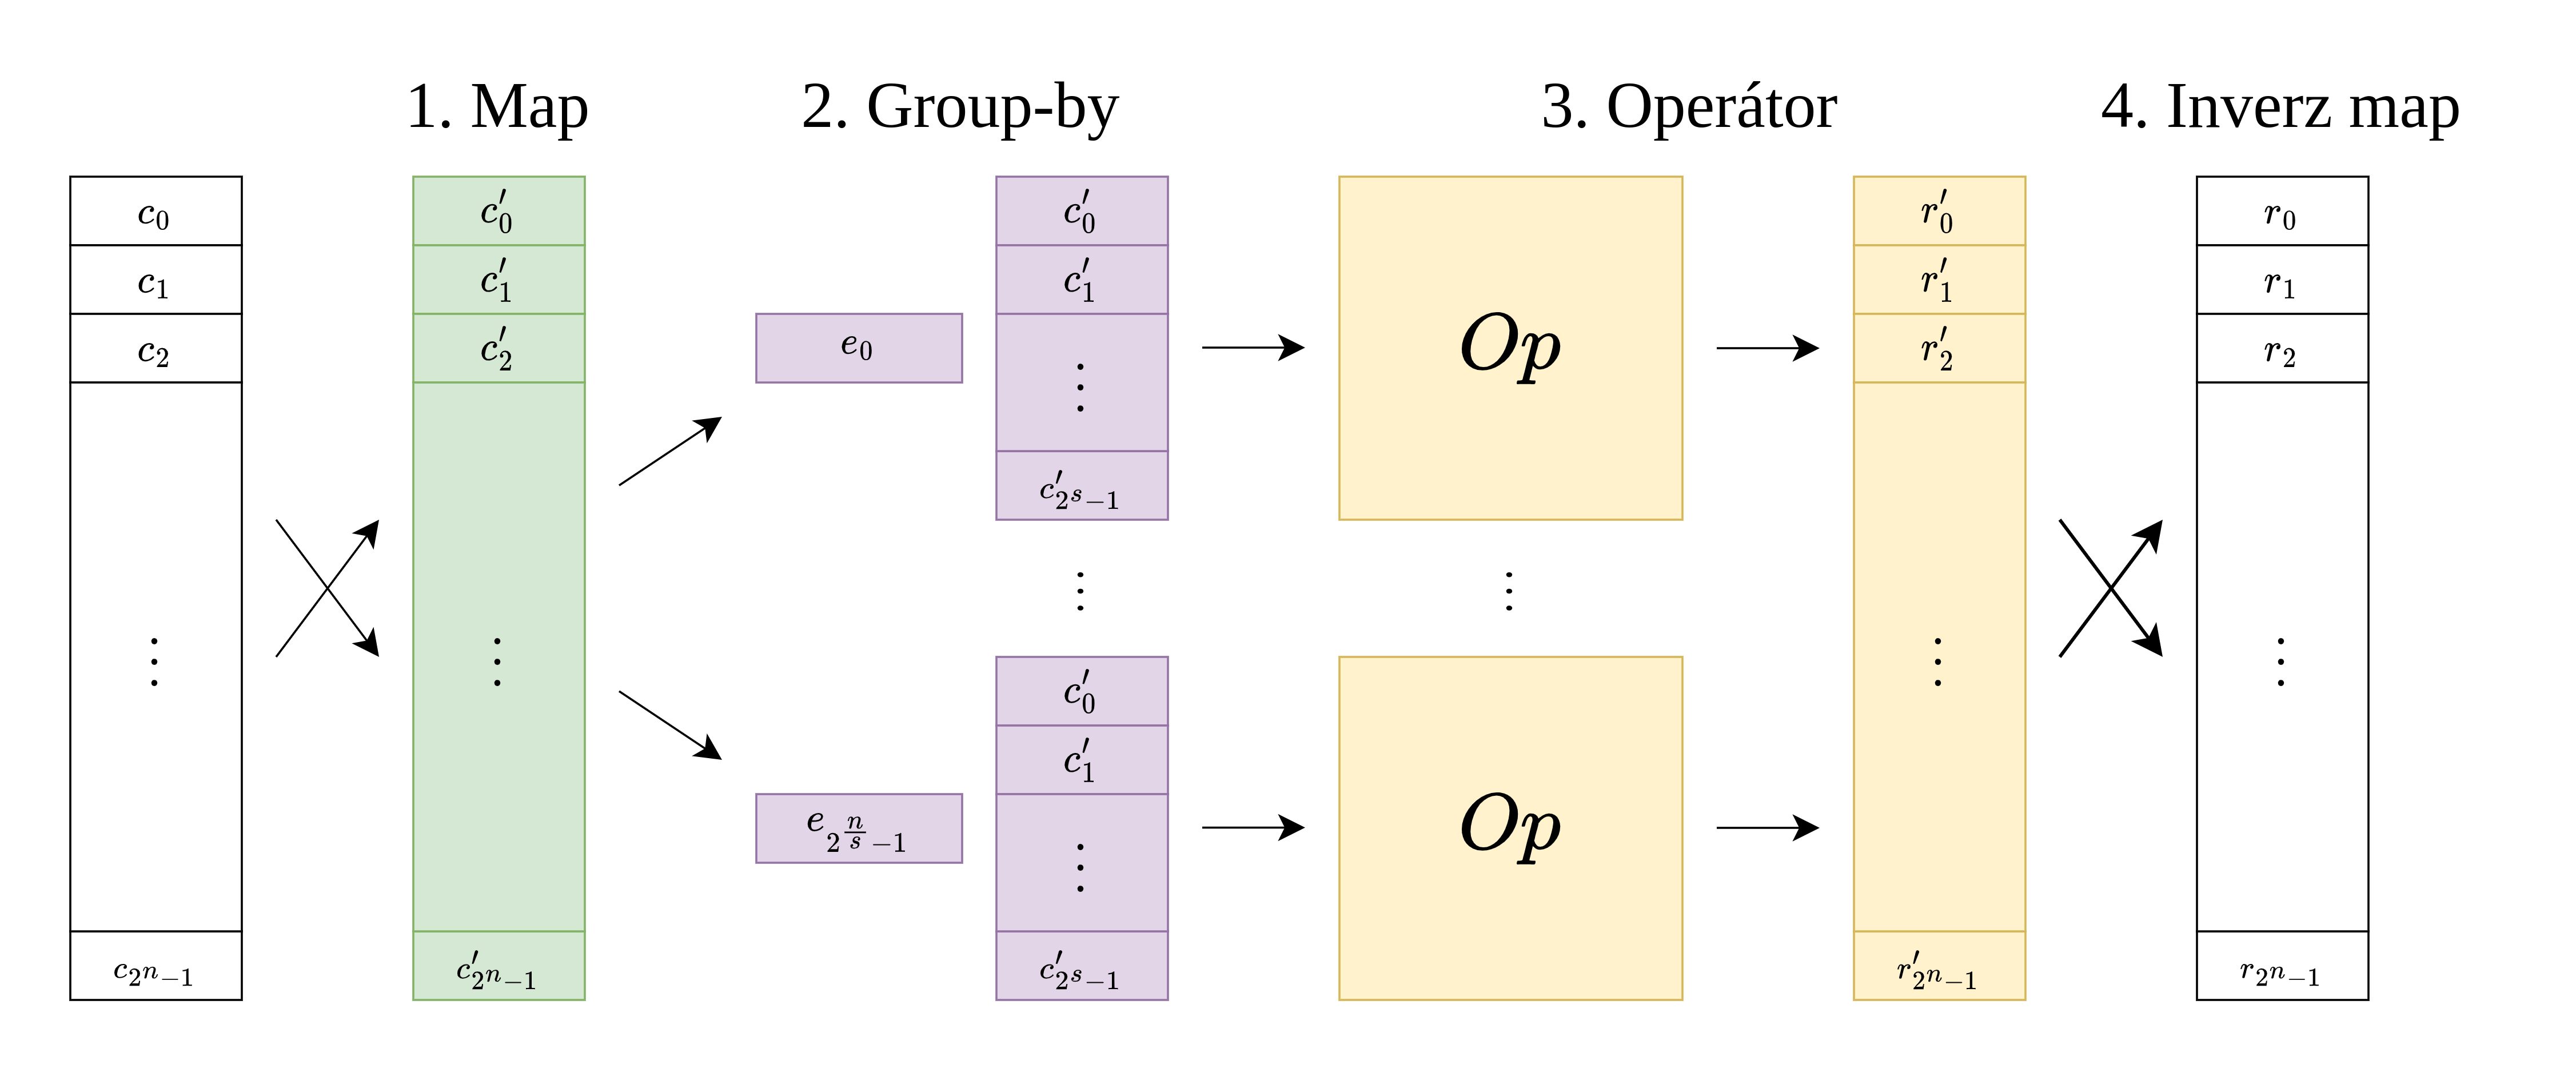
\includegraphics[width=\textwidth]{figures/qubit_map_group_by.png}
\end{figure}

\end{frame}

\begin{frame}{Operátorok megvalósítása}

Megvalósítás:

\begin{itemize}
    \item Visitor minta (inverzió):
    \begin{itemize}
        \item Operátornak odaadom a regisztert, végrehajtja magát rajta.
        \item Belső működés eltakarva: mátrix reprezentáció nem szükséges.
    \end{itemize}
    \item Strategy minta:
    \begin{itemize}
    \item Egységes algoritmus interfész: több lehetséges implementáció.
    \end{itemize}
    \item Operátor csak egy handle, példány nem foglal memóriát.
\end{itemize}

Végrehajtás:
\begin{itemize}
    \item "On-the-fly" operátorok:
    \begin{itemize}
        \item A mátrix egy sorát generálom $\rightarrow$ skalárszorzás.
        \item Hadamard, Grover.
    \end{itemize}
    \item "Függvény-alapú" operátorok:
    \begin{itemize}
        \item $u: \ket{0\dots{}0,\text{in}} \rightarrow \ket{\text{out},\text{in}}$
        \item Sum: $\sum: \ket{0\dots{}0,\text{in}} \rightarrow \ket{\text{count}(\text{in}),\text{in}}$
        \item MC-NOT: $\text{mcnot}: \ket{0,\text{in}} \rightarrow \ket{\text{any}(\text{in}),\text{in}}$
    \end{itemize}
\end{itemize}


\end{frame}

\begin{frame}{Összegzés}

\begin{itemize}
\item Eredmények:
\begin{itemize}
    \item Ritka mátrixosan tárolt regiszterek.
    \item Regiszterkezelés tetszőleges célregiszterekkel.
    \item ''On-the-fly'' operátorok: Hadamard, Grover.
    \item ''Függvény-alapú'' operátorok: Sum, Multi-Controlled NOT.
    \item Könnyű bővíthetőség új operátorral.
\end{itemize}
\item Jövőbeli terv:
\begin{itemize}
    \item Protein folding algoritmus implementálása.
    \item Döntési fa alapú tárolás kipróbálása.
\end{itemize}
\end{itemize}

\end{frame}



\begin{frame}{Bíráló kérdései - 1.}

A dolgozat bevezetésében írja, hogy az egyik motivációt a munkához a bioinformatika adja, ezen belül is a fehérje feltekeredés (protein folding) vizsgálata.

A dolgozatban azonban - érthető okokból - egy egyszerűbb problémával, a Sudoku általános változatával dolgozik.

Mégis, meg tudná mondani, hogyan lehetne (milyen jellegű továbbfejlesztésekkel) a kidolgozott eljárást a bioinformatikában használni?
\end{frame}

\begin{frame}{Bíráló kérdései - 2.}

Mi a szerző várakozása a kifejlesztett keretrendszer működési korlátait illetően?

Például:

Hány qubites Grover-keresést fog tudni implementálni?
\begin{itemize}
  \item 30 qubit körüli.
\end{itemize}
Mekkora n esetén tudja implementálni a Sudoku verifiert?
\begin{itemize}
  \item $3\times{}3$-mas Sudoku táblát lehet ($27$ qubit) $\Leftrightarrow$ $4\times{}4$-es táblát már nem ($64$ qubit).
\end{itemize}
A maximális méretű problémát implementáló kód mennyi idő alatt fog lefutni egy laptopon?
\begin{itemize}
  \item A tároláshoz $27$ qubitre + $1$ orákulum kimeneti qubitre van szükség.
  \item Az orákulum implementálása ''Függvény-alapú'' operátorral megoldható.
  \item Becsléseim szerint egy-két napon belül lefutna.
  \item Qiskit-ben ezt elkészítettem, ott a $3\times{}3$-mas Sudoku táblához $67$ TB memóriára lenne szükség.
\end{itemize}
\end{frame}

\begin{frame}{Bíráló kérdései - 3.}
A keretrendszer struktúrájában vagy implementációjában meg kell-e különböztetni a CPU-n és a GPU-n való futtatás esetét?
\begin{itemize}
  \item "On-the-fly" típusú operátorok könnyen implementálhatóak GPU-n, a meglévő keretrendszerben.
  \item "Függvény-alapú" operátorok nem vihetők át GPU-ra (nincs skalárszorzás) $\rightarrow$ sokszálú CPU-val párhuzamosíthatók.
\end{itemize}
\end{frame}

\begin{frame}{Bíráló kérdései - 4.}

Valódi kvantumszámítógépekben a kvantumbitek és a környezet kölcsönhatása dekoherenciához vezet.

A Grover-keresés működőképes marad-e, ha a dekoherenciát figyelembe vesszük a szimuláció során?
\begin{itemize}
  \item A dekoherencia csökkenti a találati valószínűséget.
  \item Amíg ez nem lép túl egy korlátot, addig többszöri ismételt futtatással javítható.
\end{itemize}
Lehetséges-e a dolgozatban kifejlesztett hatékony keretrendszert általánosítani dekoherencia jelenléte esetére, és ha igen, akkor meg lehet-e ezt tenni úgy hogy a hatékonyság is megmarad?
\begin{itemize}
  \item A dekoherencia modellezhető bizonyos valószínűséggel alkalmazott mátrixműveletekkel, ezek operátorként megvalósíthatók ebben a rendszerben.
\end{itemize}

\end{frame}

\end{document}